\documentclass[12pt,a4paper,openright,twoside]{book}
\usepackage[utf8]{inputenc}
\usepackage{phd-thesis}

\mainlinespacing{1.241} % line spacing in mainmatter, comment to default (1)

\begin{document}
	
\frontmatter
%!TeX root = phd-thesis.tex
\title{Title}
\author{Candidate Name Here}
\date{\today}

\newgeometry{margin=0.8in}
\begin{titlepage}
	\begin{center}
		% \vspace*{0.2cm}

		\large
		\textbf{ALMA MATER STUDIORUM -- UNIVERSITÀ DI BOLOGNA \\ DISI Dipartimento di Informatica: Scienza e Ingegneria}
		\\
		\noindent\hrulefill
		\vspace{0.4cm}

		\Large
		Dottorato di Ricerca in \\
		Computer Science and Engineering

		\vspace{0.4cm}

		Ciclo XXXVIII

		\vspace{0.4cm}

		Settore Scientifico Disciplinare: ING-INF/05

		Settore Concorsuale: 09/H1

		\Huge
		\vspace{3cm}
		\textbf{
			Your Fancy Title Here
		}

		{\Large{
		\vspace{3cm}

		\textit{Candidato:\\}
		\centering
		Dott. Matteo Magnini}
		\\}
		\large
		\vspace{2.5cm}
		\begin{minipage}[t]{0.64\textwidth}
			\begin{flushleft}
				\textit{Coordinatrice Dottorato:}
				\\
				\textbf{Prof.ssa Ilaria Bartolini}
			\end{flushleft}
		\end{minipage}
		\begin{minipage}[t]{0.34\textwidth}
			\begin{flushright}
				\textit{Supervisore:}
				\\
				\textbf{Prof.} \textbf{Andrea Omicini}
				\\
				\vspace{0.4cm}
				\textit{Co-supervisore:}
				\\
				\textbf{Prof.} \textbf{Enrico Denti}
			\end{flushright}

		\end{minipage}\\

		\vfill
		\noindent\hrulefill
		\vspace{0.3cm}
		\Large

		Esame finale anno 2025
	\end{center}
\end{titlepage}
\restoregeometry

\begin{abstract}
    %
    \Ac{AI} represents one of humanity's most transformative technological advancements, with roots in the mid-20th century and a rapidly growing impact on society.
    %
    Over the past decade, the field of \ac{NeSy} \ac{AI}, which seeks to integrate \emph{symbolic} and \emph{sub-symbolic} approaches, has gained increasing prominence as a promising paradigm for building intelligent systems.
    %
    By combining the structured reasoning capabilities of symbolic AI with the adaptability and scalability of sub-symbolic methods, \ac{NeSy} aims to overcome the inherent limitations of each paradigm, paving the way for more robust and interpretable AI systems.

    Within \ac{NeSy}, two foundational areas of research are \ac{SKI} and \ac{SKE}, which provide the essential tools to design hybrid systems.
    %
    \Ac{SKI} focuses on injecting structured knowledge into sub-symbolic models, enabling them to leverage prior domain expertise.
    %
    \Ac{SKE}, on the other hand, facilitates the extraction of human-understandable knowledge from these models, bridging the gap between their internal representations and user interpretability.
    %
    Together, these methods offer a pathway toward developing systems that are explainable, reliable, and effective in dynamic, real-world scenarios.

    This thesis explores the challenges and opportunities of \ac{NeSy} \ac{AI}, with a particular focus on \ac{SKI}, \ac{SKE}, and their role in the engineering of intelligent systems.
    %
    After an overview of the background and state of the art, we identify key challenges in integrating symbolic and sub-symbolic paradigms.
    %
    We then present original contributions in the form of methodologies, algorithms, and tools designed to advance the capabilities of \ac{NeSy} systems.

    The advent of \acp{LLM} has further transformed the landscape of \ac{AI}, offering unprecedented capabilities for understanding and generating natural language.
    %
    This thesis investigates how \acp{LLM} can augment \ac{SKI} and \ac{SKE}, providing new avenues for designing systems that learn and adapt autonomously.
    %
    By leveraging these models, we demonstrate how hybrid approaches can address complex challenges, such as fairness and decision-making in healthcare, while ensuring interpretability and alignment with ethical principles.

    Finally, we discuss how these advancements align with the broader vision of \ac{NeSy}, while also contributing to the specific goal of this thesis: enabling the development of systems capable of fully autonomous learning.
    %
    These systems integrate the structured reasoning of symbolic AI with the adaptability of sub-symbolic models and the transformative potential of \acp{LLM}, opening pathways toward more versatile and intelligent applications.
    %
    Such progress not only advances the field but also hints at the distant horizon of general AI, bringing us closer to a future where machines can learn, reason, and adapt autonomously.

    \sloppypar
    \textbf{Keywords} -- \emph{\acl{AI}, \acl{NeSy} \ac{AI}, \acl{SKI}, \acl{SKE}, \aclp{LLM}, Intelligent Systems, Autonomous Learning.}
\end{abstract}



\begin{dedication} % this is optional
    %
    ``The work of each individual contributes to a totality, and so becomes an undying part of the totality.
    %
    That totality of human lives -- past and present and to come -- forms a tapestry that has been in existence now for many tens of thousands of years and has been growing more elaborate and, on the whole, more beautiful in all that time.
    %
    % Even the Spacers are an offshoot of the tapestry and they, too, add to the elaborateness and beauty of the pattern.
    %
    [\dots] An individual life is one thread in the tapestry and what is one thread compared to the whole?
    %
    Daneel, keep your mind fixed firmly on the tapestry and do not let the trailing off of a single thread affect you.''

    ---Isaac Asimov, \emph{Robots and Empire}
    %
\end{dedication}

\begin{acknowledgements} % this is optional

\end{acknowledgements}

%----------------------------------------------------------------------------------------
\tableofcontents   
\listoffigures     % (optional) comment if empty
\lstlistoflistings % (optional) comment if empty
%----------------------------------------------------------------------------------------

\mainmatter

%! Author = matteomagnini
%! Date = 05/03/25

\begin{refsection}

%----------------------------------------------------------------------------------------
\minitoc
\chapter{Introduction}
\label{ch:introduction}
\mtcaddchapter
\minitoc
%----------------------------------------------------------------------------------------

\section{Research background and context}
\label{sec:research-background-and-context}
%
Through the course of history, humanity has experienced several socio-technological revolutions that have changed the way we live.
%
From the first industrial revolution that initiated the automation of manual labor, to the world-wide spread of computers that started the automation of processes and decision-making \sidenote{cite/talk about expert systems(?)}, we are now witnessing the \gls{AI} revolution.
%
The advent of \gls{AI} has already successfully automated cognitive tasks \sidenote{add citation to image recognition and similar}, and it is expected to go further by reaching -- and possibly surpassing -- \emph{human-level intelligence}.
%
\Gls{AI} is not a recent invention, it has been around since the 1950s.
%
The reasons why only now (in the last decade to be more precise) \gls{AI} has become ubiquitous are the presence of crucial ingredients that were missing in the past.
%
Thanks to
%
\begin{inlinelist}
    \item the enormous amount of \emph{data},
    %
    \item the improvement of \emph{memory} and \emph{computational power} -- that still follows the Moore's law --, and
    %
    \item the affordability of huge quantity of \emph{energy},
    %
\end{inlinelist}
%
\gls{AI} finally flourished again.


The first kind of \gls{AI} that was developed is \emph{symbolic}.
%
Symbolic means that there are \emph{symbols} with specific \emph{meanings} that are manipulated by algorithms.
%
Symbolic \gls{AI} follows the \emph{deductive} process of reasoning, where the system starts from a set of axioms and applies rules.
%
These kinds of \gls{AI} programs are pretty effective in well-defined domains where there are clear rules that always hold, e.g., board games,~\gls{TSP},~\gls{BWP}, etc.
%
\emph{Sub-symbolic} \gls{AI} is based on the \emph{inductive} process of reasoning.
%
Conversely to symbolic \gls{AI}, sub-symbolic \gls{AI} does not rely on symbols that have meanings for humans, but on data \emph{patterns}.
%
Programs that uses sub-symbolic \gls{AI} to solve a certain task are said to perform \gls{ML}, because a model needs to first learn from examples before being able to generalize to unseen data.
%
Sub-symbolic models like \glsplural{NN} can reach \emph{super-human performance} in pre-defined tasks like image recognition, natural language processing, etc., but they require a huge amount of data and hardware resources to be trained.


The natural evolution in \gls{AI} research is to use both symbolic and sub-symbolic approaches together in order to increase the performance and face more challenging tasks.
%
This is the idea behind \emph{\gls{NeSy} \gls{AI}}, where the deductive reasoning of symbolic \gls{AI} is combined with the inductive learning of sub-symbolic models, especially \glsplural{NN}.
%
This branch of \gls{AI} is relatively young; the first works that combined logic rules within a \gls{NN} date back to the 90s~\cite{DBLP:conf/aaai/TowellSN90,DBLP:journals/ai/TowellS94}.
%
The last past years have been quite prolific both in the design of new \gls{NeSy} techniques and in the development of intelligent systems that use them~\cite{DBLP:journals/csur/CiattoSAMO24}.


Finally, the advent of \glsplural{LLM} has further transformed the landscape of \gls{AI}, offering unprecedented capabilities for natural language (and also multimodal data) generation.
%
\Glsplural{LLM} are huge \gls{NN} models up to \emph{hundreds of billions} of parameters that are trained on a large corpus of text data.
%
Despite the outstanding performance that \glsplural{LLM} have achieved in many tasks, their output is just a probability distribution over the vocabulary, therefore it is subject to errors (e.g., \emph{hallucinations}) and biases (e.g., from training data, from prompt engineering).
%
\Glsplural{LLM} are still a great resource for \gls{NeSy} \gls{AI} because of their performance, versatility and customizability.
%
Ultimately, the rapid progress in \gls{NeSy} \gls{AI} and the dazzling evolution of \glsplural{LLM} are significantly changing our world, leading to more and more intelligent systems, and possibly to the advent of the \emph{singularity}~\cite{shanahan2015technological}.


\section{Overview and contributions}
\label{sec:overview-and-contributions}
%
Engineering \gls{AI} systems with characteristics approaching (super-)human intelligence remains an open and multifaceted challenge.
%
Humans exhibit a wide range of cognitive capabilities: they can perform \emph{deductive} and \emph{inductive reasoning}, \emph{plan}, \emph{adapt} to changing conditions, \emph{collaborate} with others, \emph{self-organize}, and \emph{acquire new knowledge} autonomously.
%
Each of these skills contributes to what we broadly refer to as intelligence.
%
Hence, a truly intelligent \gls{AI} system -- particularly one aiming toward \gls{AGI} -- must exhibit at least a subset of these abilities, with the capacity to learn autonomously being among the most fundamental.


To advance toward this long-term goal, we adopt a strategy based on the progressive decomposition of the overarching challenge into concrete, tractable sub-problems.
%
These include acquiring and applying domain knowledge, reasoning under uncertainty, adapting to new tasks, and ensuring interpretability and trustworthiness, among others.
%
Rather than attempting to solve \gls{AGI} in a monolithic way, we aim to address specific foundational problems that are critical building blocks for more general intelligence.


A key insight guiding this thesis is that many aspects of intelligent behavior rely on the interplay between two complementary paradigms: symbolic and sub-symbolic \gls{AI}.
%
Sub-symbolic models -- such as those developed through \gls{ML}, including \glsplural{NN} -- excel at learning from raw data and generalizing inductively.
%
Symbolic approaches, in contrast, are grounded in explicit, human-readable structures such as logic rules or ontologies, and support deductive reasoning.
%
Humans seamlessly integrate both: they learn from examples and experience, but also reason with abstract, structured knowledge.


Bridging these two paradigms is the central objective of \gls{NeSy} \gls{AI}.
%
In this context, two processes are particularly crucial: \gls{SKI} and \gls{SKE}.
%
\Gls{SKI} refers to the \emph{injection} of symbolic knowledge into sub-symbolic models, enabling them to benefit from prior domain expertise, improve generalization, enforce constraints, and operate more reliably under limited data regimes.
%
Conversely, \gls{SKE} is the process of \emph{extracting} symbolic knowledge from trained sub-symbolic models, thus making their learned internal representations accessible, inspectable, and reusable in downstream reasoning tasks.
%
Together, \gls{SKI} and \gls{SKE} form the foundational pillars of advanced \gls{NeSy} systems, enabling a virtuous cycle in which knowledge can flow in both directions -- into and out of learning systems -- fostering transparency, adaptability, and autonomy.


This thesis investigates both theoretical and practical aspects of \gls{SKI} and \gls{SKE}, proposing new methodologies, tools, and experimental frameworks to extend their applicability.
%
By exploring how these techniques can be embedded in real-world \gls{AI} systems, including in high-stakes domains such as healthcare, we aim to contribute toward the broader objective of constructing intelligent systems that learn and reason in a human-like, autonomous, and interpretable manner.



\subsection*{Research questions}
%
\begin{questions}
    \item \emph{Are \gls{SKI} and \gls{SKE} relevant in the context of modern \gls{AI}?}

    The increasing complexity and opacity of sub-symbolic models raise urgent needs for systems that are not only accurate, but also interpretable, robust, and adaptable.
    %
    \Gls{SKI} and \gls{SKE} address these needs by enabling, respectively, the integration of prior knowledge into learning systems and the extraction of insights from them.
    %
    This research investigates the relevance and impact of these techniques in real-world scenarios, and evaluates how they contribute to broader \gls{AI} goals such as trustworthiness, efficiency, and autonomy.
    %
    \label{itm:rq0}

    \item \emph{What are the characteristics of \gls{SKI} and \gls{SKE} techniques?}

    There are different ways to perform \gls{SKI} and \gls{SKE}, depending on multiple dimensions.
    %
    From these dimensions -- such as the kind of supported sub-symbolic models, the formalism of the symbolic knowledge, the ways to inject/extract the knowledge, etc. -- it is possible to refine the main research question into more detailed sub-questions.
    %
    Ultimately, from the answers to these research questions it would be possible to define a comprehensive taxonomy of \gls{SKI} and \gls{SKE} techniques.
    %
    \label{itm:rq1}

    \item \emph{How can the effects of \gls{SKI} and \gls{SKE} be measured?}

    Accuracy and other popular metrics in \gls{ML} are not the only ones that should be considered when evaluating \gls{SKI} and \gls{SKE} techniques.
    %
    There are many other aspects that a scientist or the final user of the technology wants to know.
    %
    For instance,
    %
    how robust is the model with injected knowledge to data degradation,
    %
    how well the extracted knowledge aligns with the actual behavior of the model,
    %
    whether it is possible to reduce the size of the model by injecting knowledge without losing performance, and so on.
    %
    \label{itm:rq2}

    \item \emph{When and where should \gls{SKI} and \gls{SKE} be used?}

    Traditionally, \gls{SKE} originates from the context of \gls{XAI}, where the objective is to provide a human-understandable explanation of the model's behavior.
    %
    \Gls{SKI}, on the other hand, was introduced primarily to improve model performance.
    %
    However, both techniques have many other possible applications that deserve systematic investigation.
    %
    \label{itm:rq3}

    \item \emph{How to design and develop \gls{NeSy} \gls{AI} systems that leverage \gls{SKI} and \gls{SKE}?}

    The use of \gls{SKI} and \gls{SKE} enables a variety of new applications and research directions.
    %
    These new possibilities must be explored taking into account all the consequences and implications of the use of these techniques.
    %
    \label{itm:rq4}
\end{questions}



\subsection*{Contributions}
%
The thesis mainly contributes to the field of \gls{NeSy} \gls{AI} and software engineering.
%
In particular, it focuses on \gls{SKI} and \gls{SKE} methods and on the development of \gls{AI} systems that leverage them.
%
The \textit{fil rouge} that binds all the contributions is the goal to design and develop intelligent systems, ultimately with capabilities of \emph{autonomous learning}.
%
The contributions are manifold, and they cover different aspects of \gls{NeSy} \gls{AI} including: \gls{SKI} and \gls{SKE}, software engineering, and social-technical systems.
%
In this thesis, we present the following contributions:
%
\begin{enumerate}[label=\emph{(\roman*)}]
    \item \textbf{\gls{SKI} and \gls{SKE}}

    \begin{enumerate}[label=\emph{(\arabic*)},resume]
        %
        \item we systematically collect and organise into a taxonomy \gls{SKI} and \gls{SKE} methods and technologies (\Cref{itm:rq0,itm:rq1});
        %
        \item we design, implement and validate new \gls{SKI} and \gls{SKE} methods (\Cref{itm:rq1,itm:rq3});
        %
        \item we define new metrics to evaluate the performance of \gls{SKI} techniques (\Cref{itm:rq2,itm:rq3}).
        %
    \end{enumerate}
    %
    \item \textbf{Software engineering}

    \begin{enumerate}[label=\emph{(\arabic*)},resume]
        %
        \item we design and develop software libraries to support the development and integration of \gls{SKI} and \gls{SKE} methods in \gls{AI} systems (\Cref{itm:rq4});
        %
        \item we design and develop \gls{NeSy} \gls{AI} systems that leverage \gls{SKI} and \gls{SKE} techniques in real-world scenarios (\Cref{itm:rq0,itm:rq3,itm:rq4});
        %
    \end{enumerate}
    %
    \item \textbf{Social-technical systems}

    \begin{enumerate}[label=\emph{(\arabic*)},resume]
        %
        \item we investigate how \gls{SKI} techniques can be used to mitigate the risk of bias in \gls{AI} systems (\Cref{itm:rq0,itm:rq3,itm:rq4});
        %
    \end{enumerate}
    %
\end{enumerate}


\section{Structure of the thesis}
\label{sec:structure-of-the-thesis}
%
This thesis is structured as follows.
%
\Cref{ch:introduction} sets the table, providing the background and context of the research, the research questions, and the contributions.
%
It also provides an overview of how the thesis is organised.


\Cref{part:background} gives the background necessary to understand all aspects of the research.
%
In \Cref{ch:intelligent-systems} where we introduce the broad topic of \emph{intelligence}, starting from its declinations in living beings and then going deep into machines.
%
A considerable part of the chapter is dedicated to \emph{symbolic} and \emph{sub-symbolic} \gls{AI} (\Cref{subsec:symbolic-ai,subsec:sub-symbolic-ai}), which is one of the main focus of this thesis.
%
\Cref{ch:nesy-ai} follows with a presentation of \gls{NeSy} \gls{AI}, with particular focus to \gls{SKI} and \gls{SKE} by providing a comprehensive taxonomy of the existing methods (\Cref{subsec:ski,subsec:ske}).


\Cref{part:engineering-of-ski-ske} presents one of the main contributions of the thesis.
%
\Cref{ch:ski-methods-and-contributions} introduces new \gls{SKI} methods that we designed and implemented.
%
\Cref{ch:psyki} presents \gls{PSyKI}, a software library that we developed to support the design and development of \gls{NeSy} \gls{AI} systems that leverage \gls{SKI} techniques.
%
\Cref{ch:fairness-through-ski} investigates how \gls{SKI} techniques can be used to mitigate bias in \gls{AI} systems, thus contributing to the development of \gls{TAI}.


\Cref{part:engineering-of-intelligent-systems} presents \gls{NeSy} \gls{AI} systems that leverage \gls{SKI} and \gls{SKE} techniques.
%
\Cref{ch:nesy-ai-for-real-world-applications} presents three applications of \gls{NeSy} \gls{AI} systems that we designed and developed.
%
In \Cref{ch:autonomous-learning-systems} we discuss how \gls{SKI} and \gls{SKE} techniques can be used to design and develop \gls{AI} systems with capabilities of \emph{autonomous learning}, thus contributing to the long-term goal of \gls{AGI}.

Finally, in \Cref{ch:conclusions} we summarise the main findings of the research, discuss its limitations, and outline directions for future work.



\printbibliography[title=Reference,heading=bibintoc]

\end{refsection}

%----------------------------------------------------------------------------------------
%--------------------------------------- PART I -----------------------------------------
%----------------------------------------------------------------------------------------

\part{Background}\label{part:background}

%! Author = matteomagnini
%! Date = 05/03/25

%----------------------------------------------------------------------------------------
\chapter{Intelligent Systems}
\label{ch:intelligent-systems}
\mtcaddchapter
\minitoc
%----------------------------------------------------------------------------------------

\section{What is intelligence?}\label{sec:what-is-intelligence}

Intelligence is a concept that encompasses a wide range of abilities and characteristics of single \emph{individuals} or \emph{groups}.
%
From an \emph{evolutionary} perspective, intelligence characterises some animal species -- and organisms belonging to other biological kingdoms -- from simple forms of life.
%
In the history of our planet, carbon-based life evolved from unicellular organisms to multicellular organisms, and ultimately to complex organisms with specialized cells and tissues.
%
Some of these organisms (e.g., insects) developed skills -- such as \emph{navigation}, \emph{communication}, \emph{self-organisation}, \emph{adaptation}, and so on -- that \emph{are perceived} as intelligent abilities.
%
More evolved individuals (e.g., mammals) developed even more complex forms of intelligence, such as \emph{planning}, \emph{reasoning}, \emph{learning}, etc.


In much more recent history, the carbon-based life was not the only one to ``manifest'' intelligent behaviours.
%
With the invention of the computer, also machines can perform tasks that we consider intelligent.
%
To distinguish between the intelligence of living beings and that of machines, we refer to the former as \emph{natural intelligence} and to the latter as \emph{\gls{AI}}.


Intelligence originally emerged as a result of the evolutionary process and from the interaction of organisms with each others and their environment.
%
Later, we built machines that can perform tasks that require some sort of intelligent ability.
%
However, it is us -- as humans -- \emph{to attribute} the label of intelligent to someone or something and not to others.
%
Indeed, it is said that \emph{``intelligence is in the eye of the beholder''}.
%
In this sense, we can say that intelligence is not an absolute concept, but it should be considered under a relative perspective.


Giving a rigorous definition of intelligence is not a trivial task.
%
Furthermore, there is not one single shape of intelligence, but it can be declined in many different ways (e.g., \emph{emotional intelligence}, \emph{social intelligence}, \emph{spatial intelligence}, etc.).
%
In this thesis we do not stay strictly to a specific definition of intelligence, nevertheless we give a broad definition to help the reader to get more familiar some concepts that will be introduced later.
%
We adopt a definition inspired by a notorious satirical essay by Carlo Cipolla~\cite{cipolla2013allegro}.
%
In \emph{``The basic laws of human stupidity''}, the author classifies individuals into four categories based on the result of their actions:
%
\begin{itemize}
    \item \textbf{Stupid} $\rightarrow$ losses for others and for themselves;
    \item \textbf{Helpless} $\rightarrow$ benefits for others and losses for themselves;
    \item \textbf{Bandit} $\rightarrow$ losses for others and benefits for themselves;
    \item \textbf{Intelligent} $\rightarrow$ benefits for others and for themselves.
\end{itemize}
%
Now, what is a \emph{loss} or a \emph{benefit}?
%
We can see losses and benefits as the failure or success in -- fully or partially -- achieving a certain \emph{goal}.
%
With this respect we can state that:
%
\begin{definition}[Intelligent behaviour]
    \label{def:intelligence}
    an individual (or a group) has an intelligent behaviour if it is able to \textbf{perform actions} that lead to the \textbf{achievement} of a given \textbf{goal}.
\end{definition}


In this chapter, we briefly talk about intelligence in animals and humans (\Cref{subsec:intelligence-in-animals,subsec:intelligence-in-humans}).
%
Then, we introduce \gls{AI} with a focus on reasoning and learning (\Cref{sec:intelligence-in-computer-science}).
%
Finally, we focus on the core topic of this thesis: \emph{learning} and \emph{autonomous learning} (\Cref{sec:intelligence-in-computer-science,sec:autonomous-learning}).


\subsection{Intelligence in animals}\label{subsec:intelligence-in-animals}

In order to survive in their environment, animals -- but also other organisms of different kingdoms such as plants or fungi -- have developed a set of abilities and some of them are perceived as intelligent.
%
For the sake of simplicity, we will consider just to animals, but many of the concepts we will talk about can be extended to other organisms.
%
Animals have a \emph{body}, and they are \emph{situated} in the physical world.
%
Through sensory organs, they can \emph{perceive} the environment and with muscles they can \emph{interact} with it.
%
They are \emph{autonomous} individuals, i.e., they are able to perform actions without the need of an external controller.


All animals are able to keep themselves alive (\emph{self-sufficiency}) until natural death or an accident occurs.
%
In addition to self-sufficiency, animals contribute to the survival of their species generating offspring.
%
To do so, they need to navigate the environment, find food, avoid predators, reproduce, and so on.
%
\note{TODO: add more and also examples}


\subsection{Intelligence in humans}\label{subsec:intelligence-in-humans}

Humans have developed two main characteristics about intelligence that are no match for any other animals: \emph{reasoning} and \emph{learning}.

\subsubsection{Reasoning}\label{subsubsec:reasoning}
%
Logical reasoning, or simply reasoning, is a process of drawing conclusions from premises.
%
There exists three main ways of reasoning:
%
\begin{itemize}
    %
    \item \textbf{Deductive reasoning} $\rightarrow$ it is a top-down approach that starts from a general statement and derives specific conclusions.
    %
    For example, if we know that \emph{all humans are mortal} and \emph{Socrates is a human}, we can conclude that \emph{Socrates is mortal}.
    %
    Deductive reasoning can be compared to what Kahneman calls \emph{System 2} in his book \emph{Thinking, Fast and Slow}~\cite{kahneman2011thinking}.
    %
    Kahneman describes the second system as \emph{slow thinking}, which is deliberate, effortful, logical and more rational.
    %
    \item \textbf{Inductive reasoning} $\rightarrow$ it is a bottom-up approach that starts from specific observations and derives general conclusions.
    %
    For example, if we observe that \emph{the sun rises every day}, we can conclude that \emph{the sun will rise tomorrow}.
    %
    Inductive reasoning can be mapped in the \emph{System 1} -- i.e., \emph{fast thinking} -- of Kahneman, which is automatic, effortless, intuitive and emotional.
    %
    \item \textbf{Abductive reasoning} $\rightarrow$ it is a form of reasoning that starts from an observation and seeks the simplest and most likely explanation (i.e., \emph{Occam's razor}).
    %
    For example, if we observe that \emph{the grass is wet}, we can conclude that \emph{it rained last night}.
    %
    This kind of reasoning is the same that is adopted by detectives to solve crimes.
    %
    Abduction also requires the use of statistics and probabilities, and therefore it deals with uncertainty (\emph{``Once you eliminate the impossible, whatever remains, no matter how improbable, must be the truth''---Arthur Conan Doyle}).
\end{itemize}

\subsubsection{Learning}\label{subsubsec:learning}
%
\note{TODO: talk about Learning. Experience, reinforcement, share of knowledge.}



\section{Intelligence in computer science}\label{sec:intelligence-in-computer-science}

Since the automation of computation with the invention of the computer, intelligence has always been a central topic in computer science.
%
Officially, the field of \gls{AI} was born in 1956 at the Dartmouth Conference, where a group of researchers gathered to discuss the possibility of \emph{computing towards intelligence}.
%
In this section, we present how machines can perform intelligent tasks, focussing in particular on reasoning and learning.

\subsection{Reasoning}\label{subsec:reasoning}
%
\note{TODO: fill the section}

\subsection{Learning}\label{subsec:machine-learning}
%
The learning process performed by machines is called \gls{ML}.
%
\gls{ML} is a wide umbrella term that encompasses a variety of different ways of learning and different learning tasks.
%
A widely adopted definition of \gls{ML} is the one given by Tom Mitchell in 1997~\cite{DBLP:books/daglib/0087929}:
%
\begin{quote}
    \emph{``A computer program is said to learn from experience $E$ with respect to some class of tasks $T$ and performance measure $P$ if its performance at tasks in $T$, as measured by $P$, improves with experience $E$''}.
\end{quote}
%
The software component deputed to learning is referred as \emph{model}, \emph{learner} or \emph{predictor} (and possibly other names).
%
The experience $E$ can be represented as a given dataset, i.e., a collection of input data, but there could be other ways (e.g., \Cref{subsubsec:rl}).
%
The input can come in different shapes, e.g., \emph{tabular data}, \emph{images}, \emph{text}, etc.
%
Each input type is represented in different ways to be interpreted by a machine: an entry in a table is represented as a vector of features, an image is usually represented as a matrix, or a tensor, and a text can be represented as a vector of word embeddings.
%
There can be a variety of different tasks $T$ and performance measures $P$.
%
In the rest of this section, we will provide a brief overview of the most common tasks and performance measures.


The most common macro \gls{ML} tasks are:
%
\begin{itemize}
    \item \textbf{Classification} $\rightarrow$ given the input data $X={x_1, x_2, \dots, x_n}$, the task is to predict a label $y$ (a.k.a., output) from a finite set of labels $Y=\{y_1, y_2, \dots, y_m\}$.
    %
    The input is made of numerical features $x_i$ that can either be binary, categorical, or continuous.
    %
    Ultimately, the goal is to learn a prediction function $\pi^{*}: X \rightarrow Y$;
    %
    \item \textbf{Regression} $\rightarrow$ the task consists in predicting a continuous value $y$ from the input data $X$.
    %
    Similarly to classification, the goal is to learn the optimal predictor that maps the input $X$ to the output $Y$ (usually $Y=\mathbb{R}$);
    %
    \item \textbf{Clustering} $\rightarrow$ the task is to group the input data $X$ into $k$ clusters according to some strategy (e.g., usually a distance function).
    %
    A cluster is a subset of the input data $X$ that is \emph{similar to each other} and \emph{dissimilar from the data in other clusters}.
    %
    Clustering predictors can be considered as classifiers upon anonymous classes.
    %
\end{itemize}
%
To approximate $\pi^{*}$, a learning algorithm is used.
%
Depending on the type of learning algorithm, the learning process can be \emph{supervised}, \emph{unsupervised}, or \emph{reinforcement} (see \Cref{subsubsec:supervised,subsubsec:unsupervised,subsubsec:rl}).
%

\subsubsection{Supervised}\label{subsubsec:supervised}
%
A \gls{ML} process is \emph{supervised} if it is trained on a labelled dataset.
%
The training set is made of pairs $(x_i, y_i)$, where $x_i$ is the input data and $y_i$ is the corresponding label.
%
The goal of the learning process is to learn a function $f$ that maps the input data $x_i$ to the corresponding label $y_i$.
%
The function $f$ is usually a mathematical model that is trained on the training set.
%


\subsubsection{Unsupervised}\label{subsubsec:unsupervised}

\subsubsection{\Glsentrylong{RL}}\label{subsubsec:rl}

\subsection{Agents}\label{subsec:agents}
%
We will use the term software \emph{agent} (just \emph{agent} for simplicity) from now on to refer to a software process that has particular characteristics.
%
One of these is \emph{autonomy}.
%
Autonomy is the ability of an agent to act without the direct control of humans or other agents.
%
Technically speaking, an agent encapsulates its own thread of control.
%
Autonomy is not absolute, but it is a matter of degree; e.g., self-sufficiency increases the degree of autonomy of an agent.
%
Autonomy -- \emph{per se} -- does not imply intelligence.
%
For example, from a biological perspective, a cell has some degree of autonomy (e.g., it has boundaries, it interacts with the environment, etc.), but certainly we do not consider it an intelligent entity.
%
However, it is a fundamental trait of living systems and life evolved towards more and more autonomous systems.


A \emph{robot} -- i.e., an \emph{embodied agent} -- that is able to recognise when its battery is low and to recharge itself is more autonomous than a robot that needs to be recharged by a human.


\section{Autonomous learning}\label{sec:autonomous-learning}

\subsection{Intelligent agent}\label{subsec:intelligent-agent}

\subsection{\Glsentrylongpl{MAS}}\label{subsec:mas}

\subsection{Swarm intelligence}\label{subsec:swarm-intelligence}

% \subsection{\Glsentrylong{MARL}}\label{subsec:marl}

\subsection{General learning}\label{subsec:general-learning}

%! Author = matteomagnini
%! Date = 05/03/25

%----------------------------------------------------------------------------------------
\chapter[Artificial Intelligence]{\Glsentrylong{AI}}
\label{ch:ai}
\minitoc
%----------------------------------------------------------------------------------------

\section{Overview}\label{sec:ai-overview}
%
The wide range of \gls{AI} techniques used to be divided into two main categories: \emph{symbolic} and \emph{sub-symbolic} \gls{AI}.
%
The thing that distinguishes the two categories is the way they \emph{represent knowledge} and how they process it.
%
No intelligence can exist without knowledge and no computation can occur in lack of representation.
%
In the rest of the thesis, we will use the term symbolic (resp., sub-symbolic) \gls{AI} and symbolic (resp., sub-symbolic) \gls{KR} almost interchangeably.
%
Symbolic \gls{AI} is based on \emph{symbols}, which come with a \emph{meaning} and could be manipulated according to the formalism and rules of a given \gls{AI} system.
%
On the other hand, sub-symbolic \gls{AI} is based on a numerical representation -- a.k.a., sub-symbolic -- where the numbers are not directly interpretable.
%
Numbers are technically symbols, but numbers, arrays and their functions are not recognised as means for symbolic \gls{KR}.
%
According to Van Gelder~\cite{DBLP:conf/ogai/Gelder90}, in order to be considered symbolic, \gls{KR} approaches must:
%
\begin{requirements}
    %
    \item \label{itm:symbolic-req-1} involve a set of symbols;
    %
    \item \label{itm:symbolic-req-2} the symbols can be combined following a set of grammatical rules;
    %
    \item \label{itm:symbolic-req-3} elementary symbols and combinations of symbols can be assigned a meaning.
    %
\end{requirements}


\paragraph{Local vs. distributed}
%
Multidimensional arrays are the fundamental building block of sub-symbolic data representation.
%
Formally, a $D$-order array is an ordered container of real numbers, where $D$ indicates the number of indices required to access each element.
%
We refer to 1-order arrays as \emph{vectors}, 2-order arrays as \emph{matrices}, and arrays of order greater than two as \emph{tensors}.
%
In sub-symbolic tasks based on arrays, information is typically conveyed both by the values stored in the array and their position within it.
%
The dimensions of the array -- denoted as $(d_1 \times \dots \times d_D)$ -- also play a crucial role, as sub-symbolic systems are usually designed to operate on arrays of fixed shape.
%
That is, the values of $d_1, \dots, d_D$ are chosen at design time and remain unchanged thereafter.
%
This violates \Cref{itm:symbolic-req-2} above; accordingly, we define sub-symbolic \gls{KR} as the task of encoding information into rigid numeric arrays.
%
\emph{Local} and \emph{distributed} representations are two key modes for encoding data into such arrays.
%
In local representations, each entry in the array corresponds to a well-defined concept from the target domain---its semantic meaning is clear and independent.
%
In distributed representations, by contrast, individual values carry little or no standalone meaning: their interpretation depends on the configuration of values across a neighbourhood in the indexing space.
%
Consequently, while the exact location of values is largely irrelevant in local representations, it becomes essential in distributed ones.
%
Notably, distributed representations violate \Cref{itm:symbolic-req-3}, and for this reason, recent literature often labels as \emph{sub-symbolic} those predictors that rely on distributed encoding of data.


\section{Symbolic \Gls{AI}}\label{sec:symbolic-ai}
%
Symbolic \gls{AI} has been regarded as crucial since \gls{AI}'s inception.
%
Symbolic \gls{KR} offers enhanced flexibility, expressiveness, and intelligibility, being interpretable both by machines and by humans.

\paragraph{Intentional vs. extensional}
%
In formal logic, one may define concepts either \emph{extensionally} or \emph{intensionally}.
%
Extensional definitions are direct representations of data.
%
For example, the set of square numbers admits the extensional definition $\{0,1,4,9,16,\dots\}$ by listing every member explicitly.
%
Conversely, an \emph{intensional} definition is an indirect representation of data.
%
In \gls{FOL}, this corresponds to defining a relation via a formula; for instance, the set of square numbers can be defined as $\{\,x\mid \exists n\in\mathbb{Z}\,(x = n^2)\}$ which succinctly encodes an infinite extension with a single schema.
%
Recursive intensional predicates further enhance expressivity: for example, the ancestor relation can be axiomatized by $\mathit{Ancestor}(x,y)\;\Leftrightarrow\;\mathit{Parent}(x,y)\;\lor\;\exists z\,[\,\mathit{Parent}(x,z)\wedge\mathit{Ancestor}(z,y)\,]$ allowing a compact representation of an infinite set of pairs with a finite rule.
%
In formal logic, intensional definitions are prized for their ability to model potentially unbounded domains within finite logical formalisms.


\paragraph{Expressiveness vs. tractability}
%
\begin{SCfigure}
    \centering
    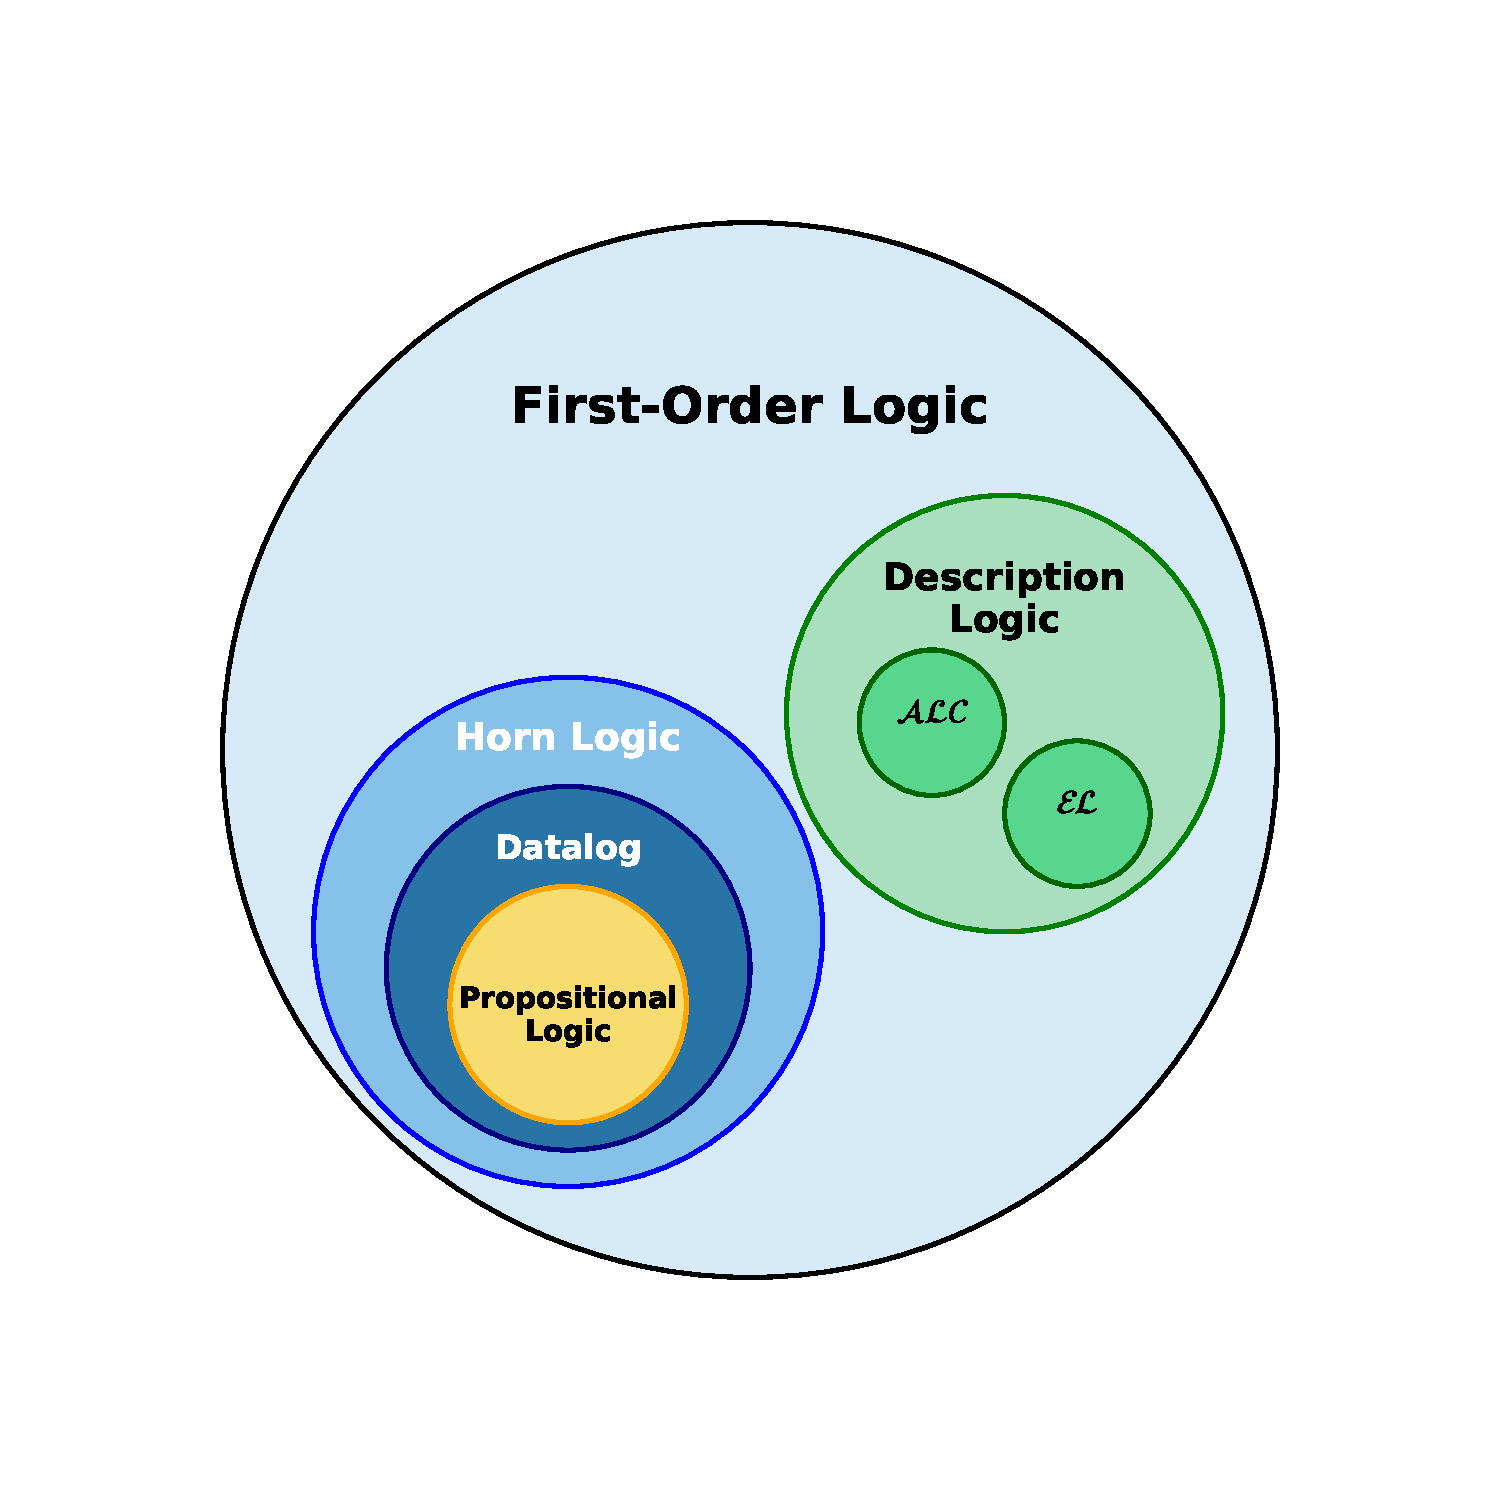
\includegraphics[width=0.58\textwidth]{figures/venn_diagram_logics}
    \caption[Venn diagram of different logic families]{
        %
        Venn diagram of different logic families, illustrating the trade-off between expressiveness and tractability.
        %
        \Gls{FOL} is the most expressive logic -- not the most expressive logic in general -- encompassing all others.
        %
        On the other hand, propositional logic is the least expressive, as it can only represent atomic propositions and their combinations.
        %
        All the other logics fall somewhere in between, with varying degrees of expressiveness and tractability.
    }
    \label{fig:venn-diagram-logics}
\end{SCfigure}

%
Tractability addresses the theoretical question of whether a logic reasoner can determine the truth of a given formula within feasible time and space bounds.
%
The answer is deeply tied to the specific reasoning algorithm and the logic's formal properties.
%
Depending on the features a logic provides -- such as quantifiers, function symbols, or recursive definitions -- it may be more or less expressive.
%
The higher the expressiveness, the more complex the problems that can be represented and reasoned about, but this also increases the computational burden.
%
This well-known phenomenon is often referred to as the expressiveness/tractability trade-off~\cite{DBLP:journals/jlp/CadoliS93,BRACHMAN2004327,DBLP:journals/ci/LevesqueB87}.
%
In practice, highly expressive logics make it easier for human users to model rich domains, often requiring fewer and more concise formulas.
%
However, this comes at the cost of automated inference, which may become computationally intractable, undecidable, or non-terminating in the general case.
%
To mitigate this issue, various fragments and extensions of \gls{FOL} have been identified, each providing different tradeoffs between what can be expressed and what can be decided efficiently.
%
\Cref{fig:venn-diagram-logics} illustrates the relationships among different logic families, highlighting the trade-off between expressiveness and tractability.


\subsection{\Glsentrylong{FOL}}\label{subsec:first-order-logic}
%
\Gls{FOL} is a general-purpose formalism that underpins most symbolic \gls{KR} systems.
%
It enables both human and computational agents to model entities and their interrelations through predicates and terms within a defined domain of discourse.
%
Its syntax comprises variables (quantified explicitly or implicitly), constants, function symbols, and predicate symbols, which are combined via logical operators such as conjunction (\(\wedge\)), disjunction (\(\vee\)), implication (\(\rightarrow\)), and equivalence (\(\leftrightarrow\)).
%
\Gls{FOL} allows for both \emph{extensional} and \emph{intensional} definitions.
%
Recursive intensional definitions, in particular, are powerful, enabling finite representations of infinite sets.
%
Despite its flexibility, \gls{FOL} is semi-decidable in general: there is no algorithm that can determine the truth of every \gls{FOL} formula in finite time, which limits its use in systems requiring guaranteed termination~\cite{DBLP:conf/dlog/2003handbook}.


\subsection{Horn logic}\label{subsec:horn-logic}
%
Horn logic is a significant subset of \gls{FOL}, offering a balanced trade-off between theoretical expressiveness and practical tractability~\cite{DBLP:journals/jcss/Makowsky87}.
%
It is built around the concept of \emph{Horn clauses}~\cite{DBLP:journals/jsyml/Horn51}, which are formulas in \gls{FOL} that exclude quantifiers and consist of a disjunction of predicates, with at most one non-negated literal.
%
Alternatively, a Horn clause can be expressed as an implication where the consequent is a single predicate and the antecedent is a conjunction of predicates: \(h \gets b_1, \dots, b_n\).
%
Here, \(\gets\) denotes logical implication (from right to left), commas represent logical conjunctions, and \(b_i\) as well as \(h\) are predicates of arbitrary arity, potentially containing \gls{FOL} terms such as variables, constants, or functions.

Horn clauses can be interpreted as \emph{if-then} rules written in reverse order, where only conjunctions of predicates are allowed in the antecedent.
%
In essence, Horn logic is a constrained subset of \gls{FOL} characterized by the following limitations:
%
\begin{inlinelist}
%
    \item formulas are reduced to clauses, containing only predicates, conjunctions, and a single implication operator;
    %
    \item operators such as \(\lor\), \(\leftrightarrow\), or \(\neg\) (negation) are not allowed;
    %
    \item variables are implicitly quantified; and
    %
    \item terms behave as they do in \gls{FOL}.
    %
\end{inlinelist}


\subsection{Datalog}\label{subsec:datalog}
%
Datalog is a declarative query language and a restricted subset of \gls{FOL}, designed for deductive databases and knowledge representation~\cite{DBLP:journals/jcss/AjtaiG94}.
%
It represents knowledge using function-free Horn clauses, as defined in \Cref{subsec:horn-logic}.
%
This restriction eliminates the use of function symbols, thereby forbidding structured terms such as recursive data structures.
%
As a result, Datalog is well-suited for applications requiring finite and decidable reasoning, as the absence of function symbols ensures termination of inference algorithms.
%
Similar to Horn logic, Datalog’s knowledge bases consist of sets of function-free Horn clauses, which are interpreted as rules and facts.
%
Rules in Datalog follow the form \(h \gets b_1, \dots, b_n\), where \(h\) is the head of the rule and \(b_1, \dots, b_n\) are the body predicates.
%
Unlike general \gls{FOL}, Datalog does not allow disjunctions, negations, or explicit quantifiers, as variables are implicitly universally quantified.
%
Datalog is widely used in areas such as \glspl{KG}, semantic web technologies, and database systems, where efficient reasoning over large datasets is required.
%
Its simplicity and computational efficiency make it a practical choice for symbolic \gls{AI} tasks that demand tractable reasoning.


\subsection{\Glsentrylong{DL}}\label{subsec:dl}
%
\Gls{DL} are a family of subsets of \gls{FOL}, typically involving limited or no quantifiers, no structured terms, and no \textit{n}-ary predicates where \(n \geq 3\)~\cite{DBLP:books/daglib/0041477}.
%
In essence, \gls{DL} represents knowledge using constants and variables, along with atomic, unary, and binary predicates.


The differences among specific variants of \gls{DL} lie in the set of supported logical connectives and whether negation is allowed.
%
The wide variety of \gls{DL} stems from the well-known trade-off between expressiveness and tractability.
%
Depending on the application, one may prefer a more expressive \gls{DL} variant, which offers richer features at the cost of reduced tractability or even decidability of algorithms manipulating the knowledge, or vice versa.


In \gls{DL}, it is common practice to use specific terminology for different elements of knowledge representation:
%
\begin{itemize}
    %
    \item Constant terms are referred to as \textit{individuals}, as each constant represents a single entity within a domain.
    %
    \item Unary predicates are called \textit{classes} or \textit{concepts}, grouping sets of individuals for which the predicate holds true.
    %
    \item Binary predicates are referred to as \textit{properties} or \textit{roles}, connecting pairs of individuals.
    %
\end{itemize}
%

Using this nomenclature, knowledge in \gls{DL} can be represented by associating entities with constants (e.g., URLs) and defining concepts and properties accordingly.
%
Binary predicates are particularly significant as they enable the connection of pairs of entities.
%
This is typically achieved through subject–predicate–object triplets, represented as ground binary predicates of the form \(\langle a \, f \, b\rangle\) or \(f(a, b)\), where \(a\) is the subject, \(f\) is the predicate, and \(b\) is the object.

Collections of such triplets form \glspl{KG}, which are directed graphs where vertices represent individuals and arcs represent binary properties connecting these individuals.
%
\glspl{KG} may explicitly or implicitly instantiate a specific ontology, which is a formal description of classes characterizing a domain, their relationships (e.g., inclusion, exclusion, intersection, equivalence), and the properties they must or must not include.


\glspl{DL} are widely used in applications such as semantic web~\cite{DBLP:conf/coopis/GangemiM03} and ontology engineering~\cite{DBLP:books/ios/HGJKP2016}, where efficient reasoning and knowledge representation are essential.
%
Their ability to balance expressiveness and computational efficiency makes them a cornerstone of symbolic reasoning systems.


\subsection{Ontologies and \glsentrylong{KG}}\label{subsec:ontologies-and-kg}
%
An ontology is a formal and explicit specification of a shared conceptualisation of a domain~\cite{DBLP:books/daglib/p/Grimm10}.
%
It provides a structured vocabulary to describe the entities relevant in that domain, along with their attributes and the relationships among them.
%
This organisation enables both human understanding and machine-based reasoning.

Ontologies are typically expressed using \glspl{DL}, a family of logic-based formalisms for knowledge representation.
%
\Glspl{DL} define three main components:
%
\begin{inlinelist}
    %
    \item\emph{concepts} (or \emph{classes}), which group entities sharing similar features;
    %
    \item\emph{individuals} (or \emph{instances}), which are the concrete elements of the domain;
    %
    \item\emph{roles} (or \emph{properties}), which describe binary relationships between individuals.
    %
\end{inlinelist}
%
Different \glspl{DL} vary in their expressive power: for example, \gls{EL} supports only conjunction and existential quantification to ensure efficient reasoning, while more expressive DLs like \gls{ALC} allow for full Boolean operators and universal quantification.

Concepts are typically denoted using capital italic letters, such as $\mathit{Animal}$ or $\mathit{Cat}$.
%
These can be combined using logical constructors like intersection ($\sqcap$), union ($\sqcup$), or negation ($\lnot$) to form more complex classes.
%
A statement like $\mathit{Cat} \sqsubseteq \mathit{Animal}$ expresses that all cats are animals.

Individuals are constants representing specific entities in the domain and are usually written in monospaced lowercase, for example \texttt{tom}.
%
Membership of an individual in a concept is denoted using the ``is-a'' relation, written as \texttt{tom}~:~$\mathit{Cat}$, meaning ``Tom is a cat.''
%
Each individual may belong to multiple concepts.

Roles represent binary relations between individuals and are written in lowercase sans-serif font, such as \textsf{eats}.
%
They connect pairs of individuals, and their domain and range can be restricted using expressions such as $\textsf{eats} \sqsubseteq \mathit{Animal} \times \mathit{Edible}$.
%
Assertions like $\textsf{eats}(\texttt{tom}, \texttt{mouse})$ state that Tom eats the mouse.

The subsumption relation ($\sqsubseteq$) is used to express inclusion between concepts or roles.
%
For instance, $\mathit{Cat} \sqsubseteq \mathit{Animal}$ means that every cat is also an animal, and $\textsf{predatorOf} \sqsubseteq \textsf{eats}$ means that every predator-prey relationship implies eating.
%
Special concepts such as $\top$ and $\bot$ are used to denote the most general and the most specific concepts, respectively.

Collections of such axioms form an ontology.
%
\Gls{TBOX} define concepts and roles and their interrelations, while \gls{ABOX} specify which individuals belong to which concepts or are related via which roles.

\Glspl{KG} also provide a structured way to represent knowledge as graphs.
%
They consist of triplets (or \emph{facts}) of the form $(s, p, o)$, where $s$ is the subject, $p$ is the predicate (or property), and $o$ is the object.
%
These triplets form a directed graph where nodes represent individuals and edges represent relationships.

Unlike ontologies, KGs do not necessarily impose formal constraints on the structure or semantics of the triplets.
%
This flexibility allows for representing heterogeneous and incomplete data.
%
However, some \glspl{KG} are explicitly grounded in an ontology, and may follow its vocabulary and logical constraints.

In summary, ontologies and knowledge graphs both aim to formally capture structured knowledge.
%
Ontologies provide formal semantics and enable logical reasoning, while knowledge graphs emphasise scalability and flexibility in representing factual data.


\subsection{Propositional Logic}\label{subsec:propositional-logic}
%
Propositional logic is a restricted subset of \gls{FOL} in which quantifiers, terms, and non-atomic predicates are absent.  
%
Its language consists solely of atomic propositions—also called 0-ary predicates—combined using standard logical connectives such as conjunction ($\land$), disjunction ($\lor$), negation ($\lnot$), and implication ($\rightarrow$).  
%
Each proposition can be interpreted as a Boolean variable that takes a truth value in \{\texttt{true}, \texttt{false}\}.  
%
The semantics of propositional logic aligns with Boolean algebra, making it straightforward to evaluate the truth of a formula given the truth values of its atomic components.

For example, a propositional formula such as $p \land \lnot q \rightarrow r$ can be interpreted as follows:  
%
$p$ might stand for the proposition ``it is raining,'' $q$ for ``there is a roof,'' and $r$ for ``the floor is wet.''  
%
In this case, the formula asserts that if it is raining and there is no roof, then the floor will be wet.

Compared to \gls{FOL}, propositional logic is significantly less expressive.  
%
The absence of quantifiers means that general statements over a domain cannot be made.  
%
Similarly, the lack of terms prevents direct reference to entities in the domain.  
%
As a consequence, each relevant aspect of a scenario must be explicitly encoded as an individual proposition.

This limitation in expressiveness has important computational implications.  
%
In particular, determining the satisfiability of a propositional formula is a decidable problem.  
%
This makes propositional logic attractive in scenarios where tractable reasoning is required.

Despite its apparent simplicity, propositional logic can model a surprising range of situations.  
%
Expressions involving numerical constants, variables, and comparisons (e.g., $x > 5$ or $y = 3$) can be encoded propositionally by introducing a distinct Boolean variable for each comparison.  
%
This reduction allows the use of propositional logic in settings where the original problem does not explicitly involve logical variables or quantifiers, but can be decomposed into atomic truth conditions.


\subsection{Limits of symbolic \Gls{AI}}\label{subsec:limits-of-symbolic-ai}
%



\section{Sub-symbolic \Gls{AI}}\label{sec:sub-symbolic-ai}
%
Sub-symbolic \gls{AI} encompasses a wide range of techniques that rely on numerical representations.
%
Contributions come from varius fields, including \gls{ML}, statistical learning, and data mining.
%
The huge number of approaches is also motivated by the well known \gls{NFL} theorem~\cite{DBLP:journals/tec/DolpertM97} that states that no single learning algorithm can outperform all others across all possible tasks.
%
The most common predictor families are linear models, \glspl{DT}, \glspl{RF}, \glspl{SVM}, \glspl{NN} (including \glspl{LLM}), and many others.


\paragraph{Predictive performance vs. interpretability}
%
\begin{figure}[h]
    \centering
    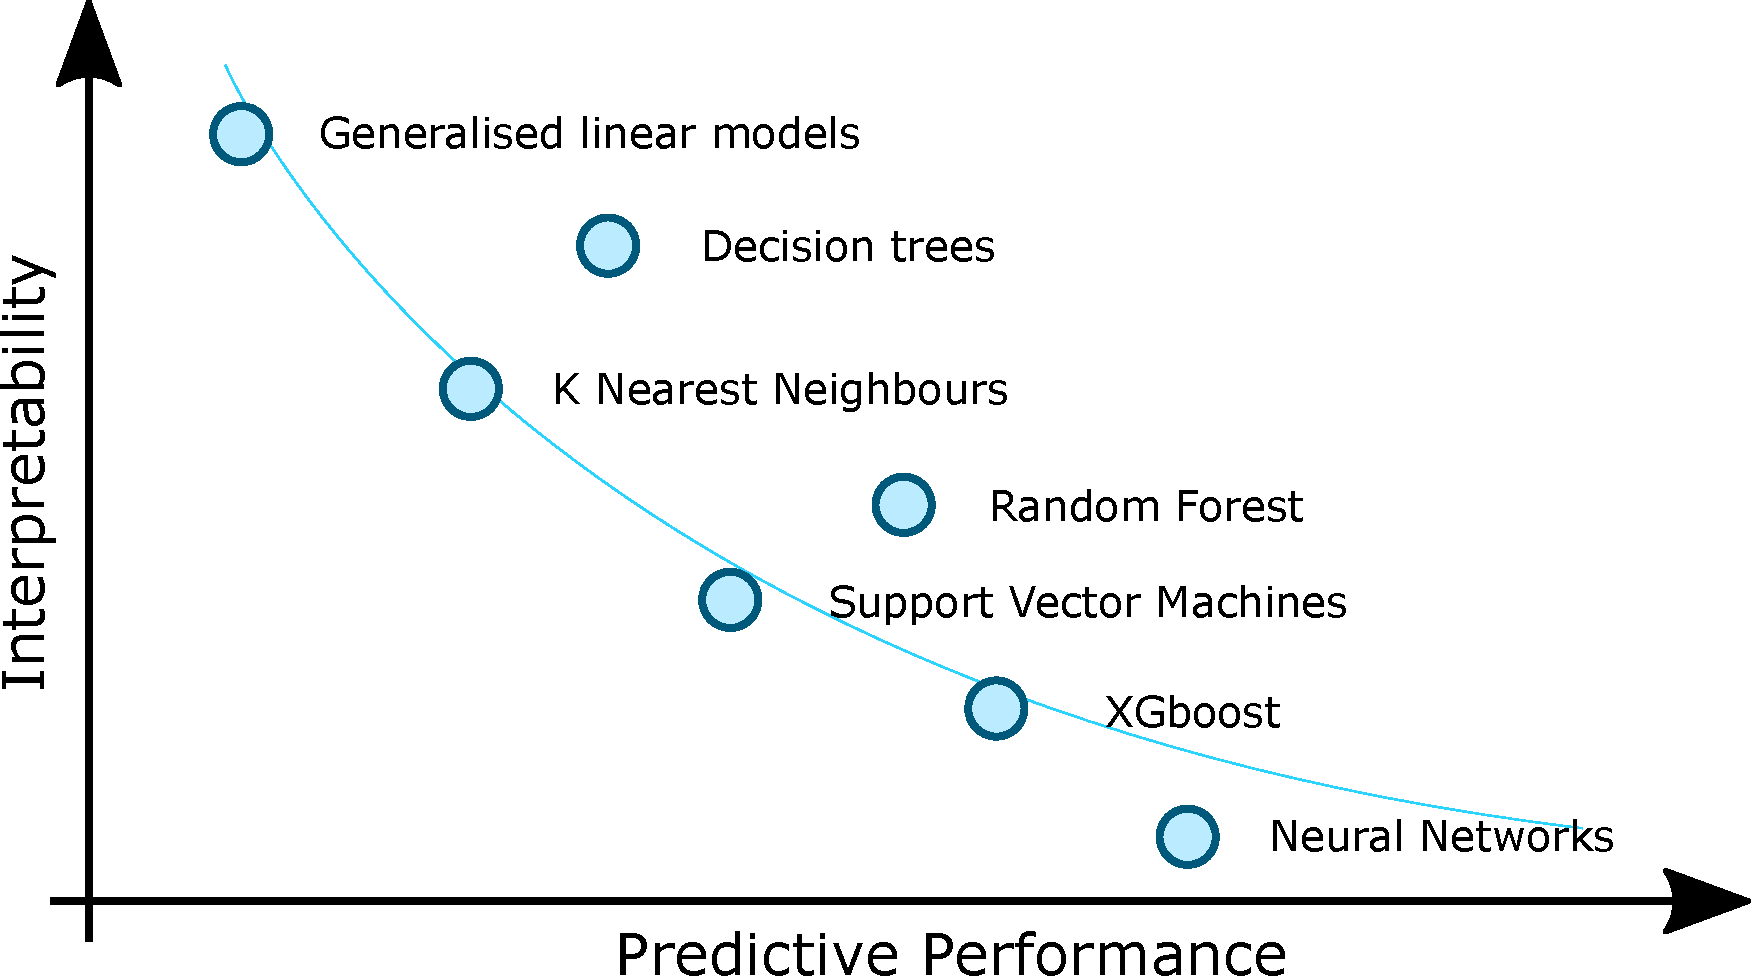
\includegraphics[width=0.9\textwidth]{figures/interpretability-performance-tradeoff}
    \caption[Performance vs. interpretability trade-off]{
        %
        Trade-off between predictive performance and interpretability in common sub-symbolic predictors.
        %
        The figure illustrates how different predictor families balance these two aspects, with simpler models being more interpretable but potentially less accurate.
        %
    }
    \label{fig:performance-vs-interpretability}
\end{figure}
%
The \emph{complexity} of a sub-symbolic predictor can vary significantly.
%
By complexity we mean the overall structure of the model, including the number of parameters, the operations that are performed, and possibly the way the model is trained.
%
\Glspl{DT}, for example, are relatively simple models that can be easily interpreted by humans.
%
The downside of \glspl{DT} is that they make predictions by linearly partitioning the input space, which can lead to poor generalisation on unseen data.
%
On the other hand, \glspl{NN} can be extremely complex, with millions of parameters and intricate architectures that are difficult to interpret.
%
However, \glspl{NN} can capture highly non-linear relationships in the data, often leading to superior predictive performance compared to simpler models.
%
The definition of interpretability is not univocal, and it lacks measures that are widely accepted~\cite{DBLP:journals/natmi/Rudin19}.
%
Despite that, \Cref{fig:performance-vs-interpretability} illustrates in an informal way the trade-off between predictive performance and interpretability in sub-symbolic predictors.


\subsection{\Glsentrylongpl{DT}}\label{subsec:decision-trees}

\subsection{\Glsentrylongpl{RF}}\label{subsec:random-forests}

\subsection{\Glsentrylongpl{SVM}}\label{subsec:svm}

\subsection{\Glsentrylongpl{NN}}\label{subsec:neural-networks}

\subsection{Limits of sub-symbolic \Gls{AI}}\label{subsec:limits-of-sub-symbolic-ai}
%! Author = matteomagnini
%! Date = 05/03/25

%----------------------------------------------------------------------------------------
\chapter{Neuro-symbolic AI}
\label{ch:nesy-ai}
\minitoc
%----------------------------------------------------------------------------------------

\section[Symbolic knowledge injection]{\Glsentrylong{SKI}}\label{sec:ski}
%
\Gls{SKI} is a wide sub-field of \gls{NeSy}, which encompasses all the methods that in some way \emph{inject} symbolic knowledge into sub-symbolic predictors.
%
More precisely, we define \gls{SKI} as:
%
\begin{definition}[\gls{SKI}]
    \label{def:ski}
    any algorithmic procedure affecting how sub-symbolic predictors draw their inferences in such a way that predictions are either \textbf{computed} as a function of, or \textbf{made consistent} with, some given symbolic knowledge~\cite{DBLP:journals/csur/CiattoSAMO24}.
\end{definition}
%
We adopt this broad definition because the amount of works in the literature is vast and varied, furthermore the contributions come from different communities (e.g., \gls{ML}, \gls{AI}, \gls{NLP}, \gls{XAI}, logics, etc.), and they often use different terminologies.


\subsection{Motivations and goals}\label{subsec:ski-motivations-and-goals}
%
\Gls{SKI} can be used for several reasons, such as:
%
\begin{inlinelist}
    %
    \item \label{itm:prediction}\emph{improving the model's predictive performance}, by leveraging symbolic knowledge to guide their learning or inference;
    %
    \item \label{itm:interpretability}\emph{improving the model's interpretability}, by making their predictions consistent with symbolic knowledge;
    %
    \item \label{itm:robustness}\emph{increase the robustness} of sub-symbolic predictors, by making them less sensitive to data perturbations (e.g., noise, data scarcity, etc.);
    %
    \item \label{itm:complexity}\emph{reduce the model complexity} of the models, by shaping their structure or by constraining their parameters;
    %
    \item and possibly many more.
    %
\end{inlinelist}


\Cref{itm:prediction} is one of the most common motivations for \gls{SKI}.
%
The idea is simple: if there is already some (symbolic) knowledge about a particular domain or task, then it is reasonable to expect that the predictor can benefit from it.
%
In this way the model learns both from the data -- inductively -- and from the symbolic knowledge---mimicking deductive reasoning.


Another common reason to use \gls{SKI} is to increase the \emph{interpretability} of the model, as stated in \Cref{itm:interpretability}.
%
In the context of \gls{XAI}, this is usually referred as \gls{XAI} \emph{by design} (\Cref{par:xai-by-design}).
%
The intuition is simple: the model is made to be consistent -- up to a certain extent -- with the symbolic knowledge, which is usually more interpretable than the model itself.
%
This can be done in two ways: either by using \emph{symbols as constraints} or by \emph{transparent box design}.
%
More details about these two approaches are provided in \Cref{subsec:learning} and \Cref{subsec:structuring}, respectively.


Predictive performances and \gls{XAI} are the main motivations for \gls{SKI}, but not the only ones.
%
The \emph{robustness} (\Cref{itm:robustness}) of a predictive model is another important challenge~\cite{DBLP:conf/eccv/LiuCZH18}, and it relates to predictors' ability to maintain performance despite the presence of input perturbations.
%
A metric of robustness in the context of \gls{SKI} is defined in the work ``An Empirical Study on the Robustness of Knowledge Injection Techniques Against Data Degradation''~\cite{DBLP:conf/woa/RafanelliMACO24}.
%
The content of the paper is presented in~\Cref{subsec:empirical-study-on-the-robustness-of-ski-methods}.
%
Along with robustness, there are other metrics -- often neglected -- that play a crucial role in the design of intelligent systems, such as \emph{memory footprint} (\Cref{itm:complexity}), \emph{latency}, data efficiency, and so on.
%
These \gls{QoS} metrics are presented in the work ``Symbolic Knowledge Injection Meets Intelligent Agents: QoS metrics and experiments''~\cite{DBLP:journals/aamas/AgiolloRMCO23}, which is discussed in~\Cref{subsec:ski-meets-intelligent-agents}.


\subsection{What to inject}\label{subsec:what-to-inject}
%
\begin{SCfigure}
    \centering
    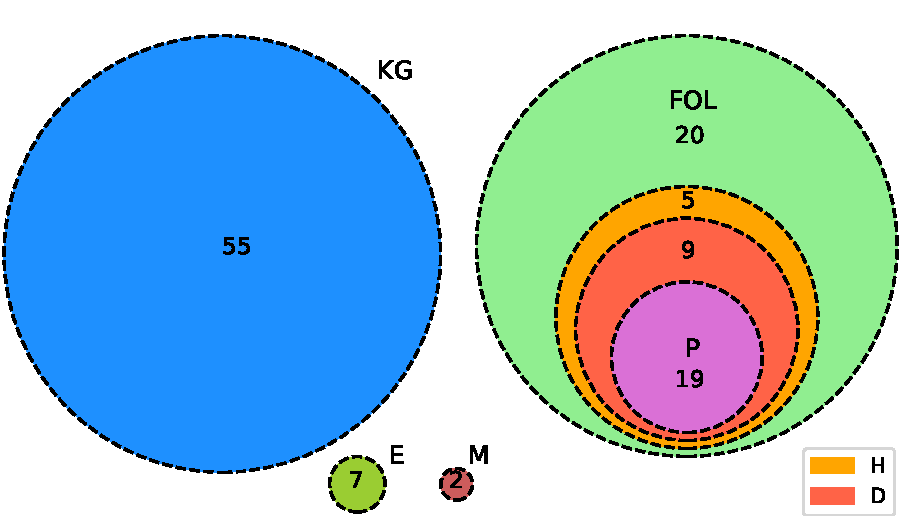
\includegraphics[width=.4\linewidth]{figures/ski-logic}
    \caption[Venn diagram categorising SKI methods]{
        Venn diagram categorising SKI methods w.r.t.\ the \emph{input knowledge} type: knowledge graphs (KG), propositional logic (P), first-order logic (FOL), expert knowledge (E), Datalog (D), Horn logic (H), or modal logic (M).
        %
        The image is taken from~\cite{DBLP:journals/csur/CiattoSAMO24} and it refers to 117 surveyed \gls{SKI} methods.
    }
    \label{fig:pie-ski-logic}
\end{SCfigure}

%
A key distinction in \gls{SKI} methods lies in whether the chosen formalism is \emph{machine interpretable}, \emph{human interpretable}, or both.
%
\Gls{SKI} methods can be categorized into two primary groups based on the formalism used to represent input knowledge~\cite{DBLP:journals/csur/CiattoSAMO24}:
%
\begin{itemize}
    \item \textbf{Logic formulas or \glspl{KB}:} These adhere to \gls{FOL} or its subsets, making them interpretable by both humans and machines.
    %
    The sub-categories, ordered by decreasing expressiveness, include:
    %
    \begin{itemize}
        %
        \item \emph{\gls{FOL} formulas:} These encompass recursive terms, variables, predicates of any arity, and various logic connectives, potentially expressing definitions.
        %
        \item \emph{Horn logic:} Often referred to as Prolog-like logic, this formalism consists of head–body rules involving predicates and terms of any kind.
        %
        \item \emph{Datalog:} A restricted subset of Horn logic that excludes recursive terms, allowing only constants or variables as terms.
        %
        \item \emph{Modal logics:} These extend the above logics with modal operators (e.g., \(\square\) and \(\lozenge\)), which express modalities such as necessity or possibility.
        %
        \item \emph{Knowledge graphs:} A practical application of description logics designed to represent entity–relation graphs.
        %
        \item \emph{Propositional logic:} This involves Boolean variables and logical connectives, offering a simpler yet effective formalism.
    \end{itemize}
    %
    \item \textbf{Expert knowledge:} This category includes human-interpretable knowledge that is not inherently machine-readable.
    %
    Examples include physics equations, syntactical rules, or domain-specific expertise.
    %
    Since expert knowledge is not directly machine interpretable, it often requires transformation into tensorial form through data generation, a process that typically involves human engineers and can be labor-intensive.
\end{itemize}
%
\Cref{fig:pie-ski-logic} illustrates the distribution of surveyed \gls{SKI} methods based on their formalism of choice.
%
\Glspl{KG} emerge as the most prevalent category, representing nearly half of the surveyed methods.
%
In contrast, modal logics constitute the smallest group.
%
Methods based on \gls{FOL} or its subsets (excluding \glspl{KG}) form another significant cluster, with propositional logic being particularly prominent due to its relative simplicity and widespread use.
%
The specific logic formalism employed in the surveyed papers is reported where available.
%
However, this information is rarely explicitly stated by the authors.
%
Instead, the logic is often inferred from the constraints and descriptions provided in the respective works.

Practical examples of symbolic knowledge that can be injected into sub-symbolic predictors are the public health guidelines on type-2 diabetes of the National Institute of Diabetes and Digestive and Kidney Diseases\footnote{\url{https://www.niddk.nih.gov/health-information/diabetes/}}.
%
These guidelines have been encoded into logic formulas~\cite{DBLP:conf/pkdd/KunapuliBSMS10} and used in works related to \gls{SKI}~\cite{Magnini-telmed2025}.
%
The first guideline state that if a patient has a glucose value greater or equal to 125 mg/dL and a \gls{BMI} greater or equal to 30, then the patient is considered diabetic.
%
The second one says that if a patient has a glucose value lower or equal to 100 mg/dL and a \gls{BMI} lower or equal to 25, then the patient is considered non-diabetic.
%
In \gls{FOL}, the first statement can be encoded as:
%
\begin{equation}\label{eq:rule-diabetic}
  \forall x . ( \text{glucose}(x) \geq 125 \land \text{bmi}(x) \geq 30 \rightarrow \text{Diabetic}(x))
\end{equation}
%
whereas the second statement can be encoded as:
%
\begin{equation}\label{eq:rule-not-diabetic}
  \forall x . ( \text{glucose}(x) \leq 100 \land \text{bmi}(x) \leq 25 \rightarrow \neg \text{Diabetic}(x))
\end{equation}


\subsection{How to inject}\label{subsec:how-to-inject}
%



\subsection{Structuring}\label{subsec:structuring}

\subsection{Learning}\label{subsec:learning}

\subsection{Embedding}\label{subsec:ski-embedding}

\subsection[Limitations and challenges of SKI]{Limitations and challenges of \Gls{SKI}}\label{subsec:limitations-and-challenges-of-ski}

\section[Symbolic knowledge extraction]{\Glsentrylong{SKE}}\label{sec:ske}

\subsection{Motivations and goals}\label{subsec:ske-motivations-and-goals}

\subsection{How to extract}\label{subsec:how-to-extract}

\subsection[Decompositional SKE]{Decompositional \Gls{SKE}}\label{subsec:decompositional-ske}

\subsection[Pedagocial SKE]{Pedagocial \Gls{SKE}}\label{subsec:pedagogical-ske}

\subsection{Local explanations}\label{subsec:local-explanations}

\subsection{Global explanations}\label{subsec:global-explanations}

\subsection[Limitations and challenges of SKE]{Limitations and challenges of \Gls{SKE}}\label{subsec:limitations-and-challenges-of-ske}
%! Author = matteomagnini
%! Date = 05/03/25

%----------------------------------------------------------------------------------------
\chapter{Large Language Models}
\label{ch:llm}
\minitoc
%----------------------------------------------------------------------------------------

\section{Architectures}\label{sec:llm-architectures}

\subsection{Transformer}\label{subsec:transformer}

\subsection{Attention}\label{subsec:attention}

\section{Fine-tuning}\label{sec:llm-fine-tuning}

\section{\Glsentrylong{RAG}}\label{sec:rag}

\subsection{Embedding}\label{subsec:rag-embedding}

\subsection{Retrieval}\label{subsec:retrieval}

\section{Limitations and challenges}\label{sec:limitations-and-challenges}

\subsection{Resources}\label{subsec:resources}

\subsection{Data and privacy}\label{subsec:data-and-privacy}

\subsection{Hallucinations}\label{subsec:hallucinations}

\subsection{Stochastic parrot or something more?}\label{subsec:stochastic-parrot-or-something-more}

%----------------------------------------------------------------------------------------
%--------------------------------------- PART II-----------------------------------------
%----------------------------------------------------------------------------------------

\part{Engineering of \ac{SKI} \& \ac{SKE}}\label{part:engineering-of-ski-ske}

\chapter{Common patterns}\label{ch:common-patterns}

\section{Knowledge representation}\label{sec:knowledge-representation}

\subsection{Logic rules}\label{subsec:logic-rules}

\subsection{\Aclp{KG}}\label{subsec:kg}

\subsection{Free text}\label{subsec:free-text}

\section{From symbolic to sub-symbolic}\label{sec:from-symbolic-to-sub-symbolic}

\subsection{Fuzzyfication}\label{subsec:fuzzyfication}

\subsection{Delegation}\label{subsec:delegation}

\section{From sub-symbolic to symbolic}\label{sec:from-sub-symbolic-to-symbolic}

\subsection{Surrogate models}\label{subsec:surrogate-models}

\subsection{De-fuzzyfication}\label{subsec:unfuzzyfication}

%----------------------------------------------------------------------------------------

\chapter{\Acl{PSyKI}}\label{ch:psyki}

\section{Implementation}\label{sec:implementation}

\subsection{Goals}\label{subsec:goals}

\subsection{Architecture}\label{subsec:architecture}

\subsection{Details}\label{subsec:details}

\section{Available \ac{SKI} methods}\label{sec:available-ski-methods}

\subsection{\Acl{KBANN}}\label{subsec:kbann}

\subsection{\Acl{KINS}}\label{subsec:kins}

\subsection{\Acl{KILL}}\label{subsec:kill}

\section{\Acl{QoS} for \ac{SKI}}\label{sec:qos}

\section{Fairness}\label{sec:fairness}

\subsection{\Acl{FaUCI}}\label{subsec:fauci}

%----------------------------------------------------------------------------------------
%----------------------------------------------------------------------------------------

\part{Engineering of intelligent systems}\label{part:engineering-of-intelligent-systems}

%----------------------------------------------------------------------------------------
%----------------------------------------------------------------------------------------

\chapter{\Ac{NeSy} \ac{AI} for real world applications}\label{ch:nesy-ai-for-real-world-applications}

\section{Motivations}\label{sec:nesy-ai-motivations}

\section{Goals and challenges}\label{sec:nesy-ai-goals-and-challenges}

\section{Applications}\label{sec:nesy-ai-applications}

\subsection{\Ac{SKE} for explainable nutritional recommenders}\label{subsec:ske-for-explainable-nutritional-recommenders}

\subsection{A general-purpose protocol for multi-agent based explanations}\label{subsec:a-general-purpose-protocol-for-multi-agent-based-explanations}

\subsection{\Acl{NeSy} \ac{AI} for supporting chronic disease diagnosis and monitoring}\label{subsec:nesy-ai-for-supporting-chronic-disease-diagnosis-and-monitoring}

\subsection{\Ac{LLM}-based solutions for healthcare chatbots: a comparative analysis}\label{subsec:llm-based-solutions-for-healthcare-chatbots-a-comparative-analysis}

\subsection{Open-source small language models for personal medical assistant chatbots}\label{subsec:open-source-small-language-models-for-personal-medical-assistant-chatbots}

\subsection{Applying \acl{RAG} on open \acp{LLM} for a medical chatbot supporting hypertensive patients}\label{subsec:applying-rag-on-open-llm-for-a-medical-chatbot-supporting-hypertensive-patients}

%----------------------------------------------------------------------------------------

\chapter{Autonomous learning systems}\label{ch:autonomous-learning-systems}

\section{Motivations}\label{sec:motivations}

\section{Goals and challenges}\label{sec:goals-and-challenges}

\section{Applications}\label{sec:applications}

\subsection{Actively learning ontologies from \acp{LLM}}\label{subsec:exact-learning-with-ac{llm}}

\subsection{\Aclp{LLM} as oracles for instantiating ontologies with domain-specific knowledge}\label{subsec:llm-as-oracles-for-instantiating-ontologies-with-domain-specific-knowledge}

%----------------------------------------------------------------------------------------

\chapter{Conclusions}\label{ch:conclusions}

\section{Discussion}\label{sec:discussion}

\section{Future work}\label{sec:future-work}

%----------------------------------------------------------------------------------------
% BIBLIOGRAPHY
%----------------------------------------------------------------------------------------

\backmatter

\part*{}

\nocite{*} % comment this to only show the referenced entries from the .bib file
\bibliographystyle{alpha}
\bibliography{phd-thesis}

\end{document}